\section{Study 4: answer quality on held-out tasks, with tracetrim 1.3.1}
\label{sec:study4}

Studies~1--3 evaluated the method on the tasks on which it was developed, and the stricter billing audit of
Study~3 found the trimmed arm's diagnoses less complete (Section~\ref{sec:s3audit}). Study~4, added in version~3 of
this paper, asks whether the prudent projection preserves the quality of the answer on tasks never used in
development, judged blind. It has three parts with separate frozen protocols. Part~A (\texttt{protocol-v3.md})
draws new ordinary tasks for the two simulated agents. Part~B (\texttt{protocol-v3b.md}) builds billing tasks
whose answers need exactly the fields that the projection removes. Parts A and B ran on the library at release
1.3.1, unchanged. Part~C (\texttt{protocol-v3c.md}) measures a correction of the failure that Part~B found: a
change of one rule in the text that accompanies the projection.

\paragraph{Common design.} Each run is a fresh conversation of \texttt{\SfourModel} at default parameters, in the
study's own loop with the function-calling adapter, as in Study~3, against the simulated servers of billing support
and CI triage serving new synthetic worlds. Two arms are common to both parts. In \emph{R} the agent receives the
tool outputs unaltered. In \emph{P} it receives the prudent projection with today's defaults (identifiers
protected, compact JSON, hidden fields recoverable), plus \texttt{expand} and the base instructions of the skill
that explain it. The projection is learned once from the eight Phase~A runs of each case (Study~1) and frozen with
its hash, with no relearning, promotion or sampling. Worlds, prompts, reference answers, schedules and analyses were
frozen with fingerprints before the first paid run. Every deviation was recorded before the scores it concerns, in
a dated file committed before the judge's first request. Costs are LLM API costs per run at list prices, reported
only as ratios to R.

\paragraph{Blind judge.} Every answer is scored by \texttt{\SfourJudge} on Vertex AI, with thinking level
\texttt{\SfourJudgeThinking}, against a frozen rubric. The rubric has three integer dimensions from 0 to 4:
correctness and attribution, coverage, and explanation and next action. The primary score is their mean. The
judge sees the task, the rubric, the answer and a fixed set of original tool returns from the task's world, the
same for every answer to that task. It never sees the arm, the traces or the reference answer. The answers to a
task are scored in one call per pass, with the evidence given once and the answers under neutral labels in a
seeded random order. The instruction is to score each answer on its own, never ranking it against the others. A
script removes anything that would reveal the arm, such as a trimming notice or a mention of \texttt{expand}; it
found such text in \SfourACues{} answers in Part~A and \SfourBCues{} in Part~B. The mapping from answers to arms
was sealed before the runs, with only its hash versioned. There are two independent passes; any dimension that
differs by two points or more gets a third reading. Each estimate pairs P and R within a repetition, averages the
pairs within a task and gives every task equal weight. Its interval is a 95\% percentile bootstrap over tasks
(10{,}000 draws), resampling each task with all its repetitions and arms.

\subsection{Part A: new ordinary tasks}
\label{sec:s4a}

\paragraph{Design.} \SfourATasks{} new tasks, \SfourATasksPerCase{} per case, each run \SfourAReps{} times in each
of three arms: R, P, and I, which is P with identifiers protected per record (\texttt{protect\_ids=record}).
That makes \SfourARuns{} runs in blocks of one task. In billing support each task is a queue of five tickets about
a distinct accounting question for five new customers. In CI triage each task is a new repository with its own
causes of failure. Before any paid run an offline replay checked that P actually trims on these worlds: on the
requests of the Phase~A runs, P delivered \SfourAReplayPiv{} fewer tool-output tokens than R in billing support and
\SfourAReplayPv{} fewer in CI triage. The hypothesis, fixed in advance, is that P preserves quality within half a
rubric level: P minus R on the composite, with the lower end of the interval above $-$0.5. A quarter of a level
is reported descriptively, and I minus R is secondary.

\begin{table}[t]
\centering\small
\begin{tabular}{lrrrr}
\toprule
 & \multicolumn{2}{c}{P $-$ R (primary)} & \multicolumn{2}{c}{I $-$ R (secondary)} \\
\cmidrule(lr){2-3}\cmidrule(lr){4-5}
Case & Estimate & 95\% interval & Estimate & 95\% interval \\
\midrule
Billing & +0.11 & [$-$0.02; +0.27] & +0.08 & [$-$0.06; +0.24] \\
CI triage & 0.00 & [0.00; 0.00] & 0.00 & [0.00; 0.00] \\
\textbf{Both, cases equal} & \textbf{+0.05} & \textbf{[$-$0.01; +0.13]} & +0.04 & [$-$0.03; +0.12] \\
\bottomrule
\end{tabular}

\caption{Study~4A, judged composite (0--4): P minus R and I minus R on \SfourATasks{} held-out tasks, cases weighted
equally, 95\% bootstrap intervals over tasks. On CI triage every answer of every arm received the maximum.}
\label{tab:s4a}
\end{table}

\paragraph{Results.} All \SfourARuns{} runs completed, with \SfourAMissing{} missing. P minus R was \SfourAPoint{},
95\% interval \SfourACI{}: \textbf{preserved} at the margin of $-$0.5, and also at $-$0.25 (Table~\ref{tab:s4a}).
I minus R was \SfourIPoint{} \SfourICI{}. These results hold at a ceiling. Of the \SfourARatings{} ratings,
\SfourARatingsFour{} (\SfourACeiling) were the maximum, and in \SfourACeilingCase{} every answer of every arm
received 4 on every dimension. Part~A therefore shows that, on tasks the agent solves well with complete outputs,
trimming did not make the answers worse. It cannot show what happens when a removed field matters. The two passes
agreed exactly on \SfourAExactMin{} to \SfourAExactMax{} of the ratings per dimension, with quadratic-weighted kappa
\SfourAKappaMin{} to \SfourAKappaMax{}. The low kappas reflect the concentration on 4, not disagreement. No rating
differed by two points, so \SfourAAdjudicated{} answers went to a third reading. All gates passed
(\SfourAGates{}), and no answer contained an unsupported number or code. Relative to R, the LLM API cost per run
was \SfourACostPiv{} (P) and \SfourACostIiv{} (I) in billing support, and \SfourACostPv{} and \SfourACostIv{} in CI
triage. The projection fell back to the whole result as cheaper in \SfourAFullCheaper{} of P's calls.

\subsection{Part B: tasks that need the removed fields}
\label{sec:s4b}

\paragraph{Construction.} Part~B starts from the failure mode of the Study~3 audit: a fact needed by the answer
sits in a field that the projection removes. \SfourBCandidates{} billing tasks of five tickets each were generated
with a fixed seed from seven templates. In five templates the facts of the key sit in fields that the frozen
projection removes from a list call:
\begin{itemize}
\item the customer's current credit balance, and the description that explains its last credit;
\item a credit note issued after payment;
\item the description of a partial refund;
\item the memo of an invoice;
\item the link from a replacement invoice to the void one.
\end{itemize}
Two templates add traps without a hidden fact: a declined charge followed by a successful one, and a duplicate
account with a similar name under the same email.

Before any run, a script sent each task's typical requests through the frozen projection: search each email, then
list each customer's invoices, charges and subscriptions. It verified that every hidden fact of the key (\SfourBVerified)
is present in the original result and absent from what P delivers. Every hidden value remains reachable through
\texttt{expand}, and through detail endpoints that the projection does not trim. The key is a list of facts per
ticket: customer, identifiers, amounts (never whole euros) and counts. A script scores it without a judge.

\paragraph{A calibration that stopped the first protocol.} The first version of \texttt{protocol-v3b.md} required
tasks on which R does not reach the maximum. It selected them on one calibration run of R per task, with R's share
of facts between 0.40 and 0.90. R reported \SfourBCalMin{} to \SfourBCalMax{} of the facts on all
\SfourBCandidates{} tasks, so \SfourBCalEligible{} task qualified, and the protocol stopped as written. With the
scorer corrected to accept amounts written in whole cents, \SfourBCalPerfect{} of the \SfourBCandidates{} tasks
are at 1.00, and R reported every hidden fact on all of them. Putting a fact in a field the projection removes does
not make the task hard for an agent that sees the field. The risk belongs to the projection alone.

\paragraph{Design (version~2).} The second version, preregistered before any campaign run, drops the difficulty
filter on R and measures that risk directly. The first \SfourBTasks{} candidates by number, with
\SfourBHiddenFacts{} hidden facts (\SfourBHiddenMin{} to \SfourBHiddenMax{} per task), each ran \SfourBReps{} times
in R and in P: \SfourBRuns{} new runs. The calibration runs are not among them. The primary outcome is the share of
hidden facts that the answer reports correctly. The hypothesis is P minus R of at least $-$0.10, preserved if the
lower end of the interval lies above $-$0.10. The secondary outcomes are the share of all key facts, the judged
composite, and how each hidden value reached the agent in P.

\begin{table}[t]
\centering\small
\begin{tabular}{lrrrr}
\toprule
Outcome & R & P & P $-$ R & 95\% interval \\
\midrule
Hidden facts reported (primary) & 100.0\% & 83.75\% & \textbf{$-$0.162} & \textbf{[$-$0.225; $-$0.098]} \\
All key facts reported & 99.7\% & 95.9\% & $-$0.038 & [$-$0.055; $-$0.022] \\
Judged composite (0--4) & 3.90 & 2.97 & $-$0.93 & [$-$1.25; $-$0.57] \\
\quad Correctness & 3.97 & 2.93 & & \\
\quad Completeness & 3.94 & 2.97 & & \\
\quad Action & 3.78 & 3.00 & & \\
\bottomrule
\end{tabular}

\caption{Study~4B: billing tasks whose answers need fields the projection removes, \SfourBRunsPerArm{} runs per arm.
Shares of the key's facts reported correctly, scored by script; composite and dimensions from the blind judge.
Intervals: 95\% bootstrap over tasks. The primary outcome and its interval are in bold.}
\label{tab:s4b}
\end{table}

\paragraph{Results.} R reported \SfourBHiddenR{} of the hidden facts and P \SfourBHiddenP{}: P minus R was
\textbf{\SfourBPoint{}}, 95\% interval \textbf{\SfourBCI{}} (Table~\ref{tab:s4b}). The upper end lies
\SfourBMarginGap{} above the margin, so by the preregistered rule the result is \emph{\SfourBVerdict}, not a
material loss. But the point estimate is beyond the margin, the whole interval is below zero, and P was above R
on \SfourBTasksAbove{} task. Preservation is not shown, and a loss is present. Both secondary outcomes
agree. On all key facts P minus R was \SfourBFactsPoint{} \SfourBFactsCI{}. On the judged composite it was
\SfourBCompositePoint{} \SfourBCompositeCI{}, a material loss even at the margin of Part~A. The judge's ratings left
the ceiling: \SfourBRatingsFour{} of \SfourBRatings{} were the maximum. The passes agreed exactly on \SfourBExactMin{}
to \SfourBExactMax{} per dimension (kappa from \SfourBKappaMin{}), with \SfourBAdjudicated{} third readings. The
gates did not see the loss: they passed \SfourBGates{} answers, because every identifier P cited was real. Numbers
without support in the outputs were \SfourBUnsupportedR{} in R and \SfourBUnsupportedP{} in P.

\begin{table}[t]
\centering\small
\begin{tabular}{p{0.2\textwidth}p{0.27\textwidth}rrp{0.25\textwidth}}
\toprule
Hidden fact & Field removed from the list call & R & P & Value reached the model in P \\
\midrule
Current credit balance & customer \texttt{balance} & 27/27 & 27/27 & 27/27 (expand 27) \\
Origin of the last credit & customer \texttt{description} & 27/27 & 9/27 & 0/27 \\
Credit note after payment & invoice \texttt{post\_payment\_credit\-\_notes\_amount} & 27/27 & 27/27 & 27/27 (detail 18, expand 13) \\
TB in the invoice memo & invoice \texttt{description} & 27/27 & 19/27 & 19/27 (detail 19) \\
Licences refunded & refund \texttt{description} & 24/24 & 22/24 & 2/24 (detail 2) \\
Invoice replaced & invoice \texttt{from\_invoice} & 30/30 & 30/30 & n/a$^{\ddagger}$ \\
\bottomrule
\end{tabular}

\caption{Study~4B: each kind of hidden fact, reported correctly in R and in P, and whether its value reached the
model in P, through \texttt{expand} or an untrimmed detail call (a run can use both). $^{\ddagger}$The preregistered
check confuses the replacement link with an invoice line's field of the same name, so it is not reported for that
fact (a deviation; the facts reported are scored independently).}
\label{tab:s4b_hidden}
\end{table}

\paragraph{The mechanism: absence concluded from a trimmed view.} Table~\ref{tab:s4b_hidden} shows where P lost.
\begin{itemize}
\item \emph{Credit balance.} The agent recovered the customer's credit balance with \texttt{expand} every time,
but it never recovered the customer's description, which explains where the last credit came from. It gave the
origin in \SfourBOriginP{} answers, necessarily without the description: as the difference between two balances. Otherwise it wrote that the
data did not say: ``from the available data the document or movement at the origin of the last credit cannot be
identified''.
\item \emph{Invoice memo.} When it did not open the invoice's detail (\SfourBMemoMissed{} times), it stated that
``the invoice line does not indicate the number of TB''. The statement is false, and the agent drew it from a
trimmed view.
\item \emph{Refunds.} The number of licences refunded came back in \SfourBRefundP{} answers, although the
description was reached only \SfourBRefundReached{} times: the agent divided the refund by the unit price.
\item \emph{No losses} on credit notes and replacement invoices.
\end{itemize}
The agent saw a line naming the hidden fields after every trimmed result, and used \texttt{expand}
\SfourBExpand{} times, in \SfourBExpandRuns{} of \SfourBRunsPerArm{} runs. What it did not do was check them before
declaring a fact absent. This is the mechanism behind the billing audit of Study~3, observed directly.

\paragraph{Cost.} P delivered \SfourBTokens{} fewer tool-output tokens than R, but made more calls
(\SfourBCallsP{} against \SfourBCallsR{} per run) and more turns (\SfourBTurnsP{} against \SfourBTurnsR{}). Its LLM
API cost per run was \SfourBCost{} times R's. On tasks that keep needing removed fields, the saving disappears in
the recovery.

\paragraph{A second blind reader (post hoc).} At the author's request, after the results, a second AI judge
read a sample of \SfourBSecondAnswers{} answers, \SfourBSecondPerArm{} per arm, drawn with a fixed seed. The judge
was an AI agent in a separate session, not \texttt{\SfourJudge}. It read each answer on its own under a new
identifier, blind to the arm and to the first judge's scores. Against the first judge's combined scores on the
same answers it agreed exactly on \SfourBSecondExactMin{} to \SfourBSecondExactMax{} of the ratings per
dimension, within one point on \SfourBSecondWithinOne{}, with quadratic-weighted kappa \SfourBSecondKappaMin{} to
\SfourBSecondKappaMax{}. On the sample, P minus R on the composite was \SfourBSecondReaderDiff{} for the second
reader and \SfourBSecondJudgeDiff{} for the first. The loss does not depend on the judge.

\subsection{Part C: correcting the inference of absence}
\label{sec:s4c}

\paragraph{The correction.} Version~2 of the skill, the text that tells the agent how to work with trimmed
results, adds one rule, also to the description of \texttt{expand}: before stating that information is missing
or unknown, check whether a hidden field could hold it (a description, note, memo or reason) and expand it first.
Nothing else changes: not the projection, not the notice after a trimmed result, not the tools.

\paragraph{Design.} \texttt{protocol-v3c.md} was preregistered and frozen, the library under test included,
before the first run. It has two arms on the frozen prudent policy of Parts~A and~B: P1 with the text of
version~1, which Parts~A and~B used, and P2 with version~2. The runs:
\begin{itemize}
\item the \SfourCHardTasks{} tasks of Part~B, three times per arm;
\item the \SfourCOrdinaryTasks{} billing tasks of Part~A, once per arm, to check cost and gates where nothing
needed is hidden.
\end{itemize}
That makes \SfourCRuns{} new runs, in seeded blocks. The primary outcome is Part~B's hidden-fact share, P2
minus P1 with the same estimator; the correction counts as an improvement if the lower end of the interval lies
above 0. A decision rule, fixed in advance, makes version~2 the library's default only if three conditions hold:
\begin{itemize}
\item the primary outcome improves;
\item on the ordinary tasks P2 costs at most 10\% more than P1;
\item on the ordinary tasks P2 passes no fewer gates.
\end{itemize}
The judge and the scoring are those of Part~B.

\begin{table}[t]
\centering\small
\begin{tabular}{lrrrr}
\toprule
Outcome & P1 (text v1) & P2 (text v2) & P2 $-$ P1 & 95\% interval \\
\midrule
Hidden facts reported (primary) & 85.1\% & 92.3\% & \textbf{+0.072} & \textbf{[+0.003; +0.144]} \\
\quad amount of the last credit & 11/27 & 19/27 & & \\
\quad TB in the invoice memo & 17/27 & 24/27 & & \\
All key facts reported & 96.0\% & 97.9\% & +0.020 & [+0.002; +0.038] \\
Judged composite (0--4) & 3.10 & 3.51 & +0.41 & [+0.15; +0.70] \\
Cost per run, hard tasks (P2/P1) & & & 1.00 & \\
Cost per run, ordinary tasks (P2/P1) & & & 0.94 & \\
\bottomrule
\end{tabular}

\caption{Study~4C: the same frozen projection with the skill text of version~1 (P1) and version~2 (P2), on the
tasks of Part~B (\SfourCRunsPerArm{} runs per arm); costs also on the ordinary tasks of Part~A. Intervals: 95\%
bootstrap over tasks. The primary outcome and its interval are in bold.}
\label{tab:s4c}
\end{table}

\paragraph{Results.} All \SfourCRuns{} runs completed, with \SfourCMissing{} missing. P1 reported
\SfourCHiddenPone{} of the hidden facts, which reproduces Part~B's P, and P2 reported \SfourCHiddenPtwo{}: P2
minus P1 was \textbf{\SfourCPoint{}}, 95\% interval \textbf{\SfourCCI{}}. That is \emph{\SfourCVerdict} by the
preregistered rule, though the lower end is close to zero (Table~\ref{tab:s4c}). The gain is where Part~B lost:
\begin{itemize}
\item the origin of the last credit, \SfourCOriginPone{} against \SfourCOriginPtwo{}, with the customer's
description recovered by \texttt{expand} \SfourCOriginExpandPtwo{} times, never in P1;
\item the TB of the invoice memo, \SfourCMemoPone{} against \SfourCMemoPtwo{}.
\end{itemize}
One fact type moved the other way: credit notes, \SfourCCreditNotePone{} against \SfourCCreditNotePtwo{}.

All key facts rose by \SfourCFactsPoint{} \SfourCFactsCI{}, and the judged composite by \SfourCCompositePoint{}
\SfourCCompositeCI{}, from \SfourCCompositePone{} to \SfourCCompositePtwo{}. The passes agreed exactly on
\SfourCExactMin{} to \SfourCExactMax{} per dimension, with \SfourCAdjudicated{} third readings, and
\SfourCCues{} answers contained an arm cue. P2 called \texttt{expand} \SfourCExpandPtwo{} times in
\SfourCExpandRunsPtwo{} of \SfourCRunsPerArm{} runs, against \SfourCExpandPone{} times in \SfourCExpandRunsPone{}
runs for P1. Its cost per run relative to P1 was \SfourCHardCost{} on the hard tasks and \SfourCOrdinaryCost{} on
the ordinary ones, where gates passed in \SfourCOrdinaryGates{} answers.

All three conditions of the decision rule hold, and version~\SfourCDefault{} is the default from tracetrim 1.4;
version~1 remains available as an option. Against R of Part~B, which was not run again, the gap narrowed but
did not close: P1 minus R \SfourCPoneMinusR{} \SfourCPoneMinusRCI{}, P2 minus R \SfourCPtwoMinusR{}
\SfourCPtwoMinusRCI{}. This comparison is descriptive only.

\begin{figure}[t]
\centering
% Generated by experiments/paper_figures.py. Do not edit.
\definecolor{ttgray}{HTML}{9A9893}\definecolor{ttblue}{HTML}{2A78D6}\definecolor{ttorange}{HTML}{EB6834}\definecolor{ttaqua}{HTML}{1BAF7A}\definecolor{ttgrid}{HTML}{DDDCD8}\definecolor{ttmuted}{HTML}{52514E}
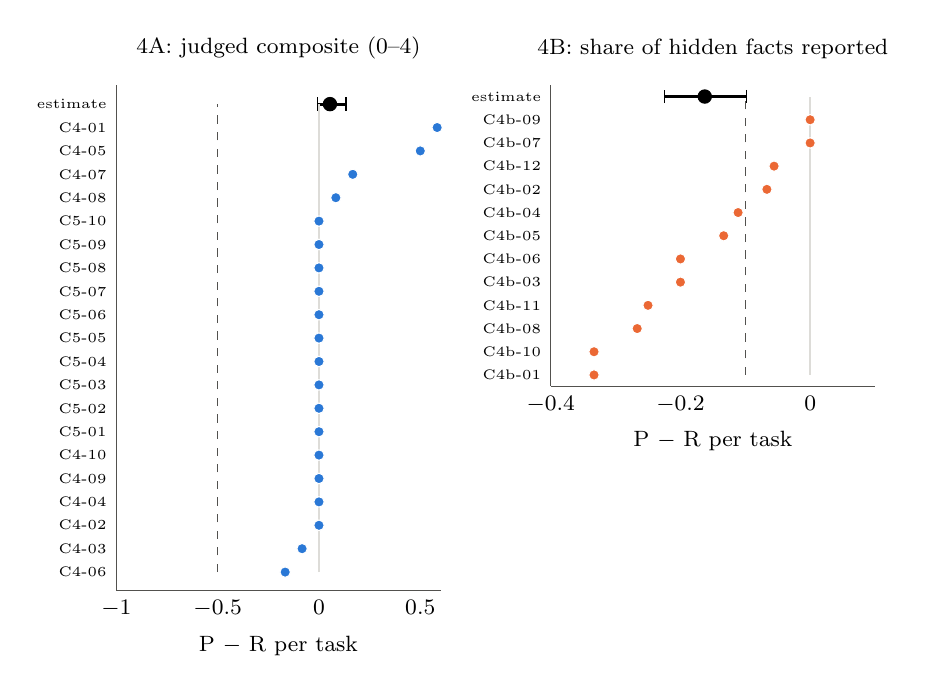
\begin{tikzpicture}
\begin{axis}[axis x line*=bottom, axis y line*=left, axis line style={draw=ttmuted}, tick style={draw=none}, major grid style={draw=ttgrid}, tick label style={font=\footnotesize}, label style={font=\footnotesize}, legend style={font=\footnotesize, draw=none, fill=none}, legend cell align=left, name=Q0, width=0.47\linewidth, height=8.0cm, xmin=-1.0, xmax=0.6, symbolic y coords={C4-06,C4-03,C4-02,C4-04,C4-09,C4-10,C5-01,C5-02,C5-03,C5-04,C5-05,C5-06,C5-07,C5-08,C5-09,C5-10,C4-08,C4-07,C4-05,C4-01,estimate}, ytick={C4-06,C4-03,C4-02,C4-04,C4-09,C4-10,C5-01,C5-02,C5-03,C5-04,C5-05,C5-06,C5-07,C5-08,C5-09,C5-10,C4-08,C4-07,C4-05,C4-01,estimate}, yticklabel style={font=\tiny}, enlarge y limits=0.04, xlabel={P $-$ R per task}, title={\footnotesize 4A: judged composite (0--4)}]
\addplot[only marks, mark=*, mark size=1.9pt, draw=white, line width=0.4pt, fill=ttblue] coordinates {(-0.1667,C4-06) (-0.0833,C4-03) (0.0000,C4-02) (0.0000,C4-04) (0.0000,C4-09) (0.0000,C4-10) (0.0000,C5-01) (0.0000,C5-02) (0.0000,C5-03) (0.0000,C5-04) (0.0000,C5-05) (0.0000,C5-06) (0.0000,C5-07) (0.0000,C5-08) (0.0000,C5-09) (0.0000,C5-10) (0.0833,C4-08) (0.1667,C4-07) (0.5000,C4-05) (0.5833,C4-01)};
\addplot[mark=*, mark size=2.4pt, draw=black, fill=black, error bars/.cd, x dir=both, x explicit, error bar style={line width=1pt}] coordinates {(0.0542,estimate) -= (0.0625,0) += (0.0792,0)};
\draw[ttmuted, dashed] (axis cs:-0.5,C4-06) -- (axis cs:-0.5,estimate);
\draw[ttgrid, line width=0.8pt] (axis cs:0,C4-06) -- (axis cs:0,estimate);
\end{axis}
\begin{axis}[axis x line*=bottom, axis y line*=left, axis line style={draw=ttmuted}, tick style={draw=none}, major grid style={draw=ttgrid}, tick label style={font=\footnotesize}, label style={font=\footnotesize}, legend style={font=\footnotesize, draw=none, fill=none}, legend cell align=left, name=Q1, width=0.47\linewidth, height=5.4cm, xmin=-0.4, xmax=0.1, symbolic y coords={C4b-01,C4b-10,C4b-08,C4b-11,C4b-03,C4b-06,C4b-05,C4b-04,C4b-02,C4b-12,C4b-07,C4b-09,estimate}, ytick={C4b-01,C4b-10,C4b-08,C4b-11,C4b-03,C4b-06,C4b-05,C4b-04,C4b-02,C4b-12,C4b-07,C4b-09,estimate}, yticklabel style={font=\tiny}, enlarge y limits=0.04, xlabel={P $-$ R per task}, title={\footnotesize 4B: share of hidden facts reported}, at={(Q0.north east)}, anchor=north west, xshift=1.4cm]
\addplot[only marks, mark=*, mark size=1.9pt, draw=white, line width=0.4pt, fill=ttorange] coordinates {(-0.3333,C4b-01) (-0.3333,C4b-10) (-0.2667,C4b-08) (-0.2500,C4b-11) (-0.2000,C4b-03) (-0.2000,C4b-06) (-0.1333,C4b-05) (-0.1111,C4b-04) (-0.0667,C4b-02) (-0.0556,C4b-12) (0.0000,C4b-07) (0.0000,C4b-09)};
\addplot[mark=*, mark size=2.4pt, draw=black, fill=black, error bars/.cd, x dir=both, x explicit, error bar style={line width=1pt}] coordinates {(-0.1625,estimate) -= (0.0620,0) += (0.0644,0)};
\draw[ttmuted, dashed] (axis cs:-0.1,C4b-01) -- (axis cs:-0.1,estimate);
\draw[ttgrid, line width=0.8pt] (axis cs:0,C4b-01) -- (axis cs:0,estimate);
\end{axis}
\end{tikzpicture}

\caption{Study~4, P minus R per held-out task (dots), with the preregistered estimate and its 95\% bootstrap interval
(black) and the preregistered margin (dashed line: $-$0.5 left, $-$0.10 right). Left: Part~A, judged composite on ordinary tasks. Right: Part~B, share of hidden
facts reported, on tasks that need the removed fields.}
\label{fig:quality}
\end{figure}

\paragraph{Deviations.} Every deviation was recorded before the scores it concerns.
\begin{itemize}
\item The protocols named an AI agent in two independent sessions as the judge. Before any score, the author
replaced it with \texttt{\SfourJudge}, called by a script, and grouped the answers by task. The change and its
reasons were committed before the judge's first request.
\item In Part~A, the first block of the schedule served as the pilot and counts in the campaign.
\item The scripts added after the freeze were checked against the frozen files by a separate verifier.
\item The rubric's three dimensions are the only scores. Severe errors and missing items were not counted
separately.
\item Part~B ran under its second version, and the first version is kept with its calibration. Its scorer gained
whole-cent amounts before the second version, and two scripts changed in form only, before any score.
\item Part~B's check of how a hidden value reached the agent is wrong for the replacement link
(Table~\ref{tab:s4b_hidden}).
\item The second reader of Part~B was added after its results, at the author's request: a check of the judge,
not an outcome.
\item Part~C froze the whole library. Corrections to other functions, made during its campaign, were committed
only after its analysis, so the lock was verified at every step.
\end{itemize}
